\documentclass[11pt, a4paper]{article}
\usepackage[utf8]{inputenc}
\usepackage{graphicx}
\usepackage{setspace}
\usepackage{array}
\usepackage{fancyhdr}
\usepackage[none]{hyphenat}
\usepackage{rotating}
\usepackage{anyfontsize}
% For subfigures
\usepackage{caption}
\usepackage{subcaption}
% Get rid of the indent of the first line
\edef\restoreparindent{\parindent=\the\parindent\relax}
\usepackage{parskip}
% Fix text out of margin
\emergencystretch 3em
% Set date format
\usepackage[ddmmyyyy]{datetime}
% Set fonts
\usepackage{fontspec}
\setmainfont{Muli}[
    Path = fonts/ ,
    Extension = .ttf ,
    UprightFont = *-Regular ,
    ItalicFont = *-Italic ,
    BoldFont = *-Bold ,
    BoldItalicFont = *-BoldItalic
]
\setsansfont{Muli-Black}[
    Path = fonts/ ,
    Extension = .ttf ,
    ItalicFont = *Italic
]
% Set page margin
\usepackage{geometry}
\geometry{a4paper,
            % total={175mm,257mm}, %space for content
            headheight=80pt,
            headsep=2pt,
            % top=3cm,
            bottom=2.5cm,
            left=2cm,
            right=1.75cm}
% Set the name of the table of contents
\usepackage{url}                                                  % for correct typesettings of URLs
\usepackage{rotating}
\usepackage{hyperref}                                             % for sophisticated linking of urls, dois, pictures, tables, etc.
\hypersetup{
    unicode=true,                                                 % non-Latin characters in Acrobat’s bookmarks
    pdftoolbar=true,                                              % show Acrobat’s toolbar?
    pdfmenubar=true,                                              % show Acrobat’s menu?
    pdffitwindow=false,                                           % window fit to page when opened
    pdfstartview={FitH},                                          % fits the width of the page to the window
    pdfauthor={C. Fortmann-Grote},                                           % author
    pdftitle={D5.3: Release of documented simulation APIs},   % title
    pdfsubject={PaNOSC WP5 (ViNYL) Deliverable D5.3},                             % subject of the document
    pdfcreator={pdflatex},                                         % creator of the document
    pdfnewwindow=true,                                            % links in new PDF window
    colorlinks=true,                                              % false: boxed links; true: colored links
    linkcolor=black,                                                % color of internal links (change box color with linkbordercolor)
    citecolor=blue,                                                % color of links to bibliography
    filecolor=blue,                                               % color of file links
    urlcolor=blue                                                 % color of external links
}
% \usepackage[style=nature]{biblatex}
% \addbibresource{references.bib}



\pagestyle{fancy}
\fancyhead{} % clear all header fields
\fancyfoot{} % clear all footer fields
\renewcommand{\headrulewidth}{0pt} % clear the header ruler line
\setlength{\footskip}{14pt}
\fancyfoot{} % clear all footer fields
\fancyfoot[R]{\hspace{1em}}
% \fancyfoot[c]{\begin{tabular}{c}
% 
\includegraphics[width=\textwidth, valign=b]{footer.pdf}& \\
% \end{tabular}}
\fancyfoot[L]{\hspace{1cm} 
\includegraphics[width=0.95\textwidth]{footer.pdf}}
% \cfoot{
\includegraphics[width=0.95\textwidth]{footer.pdf}}

% Set line spacing
\emergencystretch 3em
\setstretch{1.2}
% \setlength{\footskip}{10pt}

\begin{document}
% \thispagestyle{empty}
\chead{
\includegraphics[width=\textwidth]{header.pdf}}

{
	\centering
    \begin{onehalfspace}
    \sffamily
     \vspace*{5ex}
	{\fontsize{20}{24}\selectfont PaNOSC \par}
	{\fontsize{20}{24}\selectfont Photon and Neutron Open Science Cloud \par}
	{\fontsize{20}{24}\selectfont H2020-INFRAEOSC-04-2018 \par}
	{\fontsize{20}{24}\selectfont Grant Agreement Number: 823852 \par}
	\end{onehalfspace}

	\vspace*{7ex}
	
\includegraphics[width=\textwidth]{PaNOSClogo_web_RGB.pdf}\par
	\vfill
	{\large \textbf{\sffamily D5.3: Repository of documented jupyter notebooks and Oasys canvases}}\par
} % end of centering


\includegraphics[width=1.27in]{by.eps}\par
This work is licensed under a Creative Commons Attribution 4.0 International License\\
(\url{http://creativecommons.org/licenses/by/4.0/})\par

% \vspace*{0ex}
\newpage

% Set footer for the second page
% \setlength{\footnotesep}{50pt}
% \setlength{\footskip}{0pt}
\fancyfoot{} % clear all footer fields
\fancyfoot[R]{\thepage}
% \fancyfoot[c]{\begin{tabular}{c}
% 
\includegraphics[width=\textwidth, valign=b]{footer.pdf}& \\
% \end{tabular}}
\fancyfoot[L]{\hspace{1cm} 
\includegraphics[width=0.95\textwidth]{footer.pdf}}


{ %Front page
\restoreparindent
% \renewcommand{\arraystretch}{1.2} % change table row height

{\sffamily\huge Project Deliverable Information Sheet \par}

\begin{center}
\begin{tabular}{ | m{5.2cm}| m{10.7cm} | }
\hline
Project Reference No. & 823852 \\
\hline
Project acronym: & PaNOSC \\
\hline
Project full name: & Photon and Neutron Open Science Cloud \\
\hline
H2020 Call: & INFRAEOSC-04-2018 \\
\hline
Project Coordinator: & Andy Götz (andy.gotz@esrf.fr) \\
\hline
Coordinating Organization: & ESRF \\
\hline
Project Website: & www.panosc.eu \\
\hline
Deliverable No: & D5.3: Repository of documented jupyter notebooks and Oasys canvases \\
\hline
Deliverable Type: & Software \\
\hline
Dissemination Level: & Public \\
\hline
Contractual Delivery Date: & 30/05/2022 \\
\hline
Actual Delivery Date: & \today \\
\hline
EC project Officer: & Ren\'e Martins \\
\hline
\end{tabular}
\end{center}

{\large \textbf{Document Control Sheet} \par}
\begin{center}
\begin{tabular}{ | m{5.2cm}| @{}c@{} | }
\hline
\textbf{Document}
&
\begin{tabular}{| m{10.7cm} |}
Title: D5.3: Repository of documented jupyter notebooks and Oasys canvases \\\hline
Version: 1 \\\hline
Available at: \\\hline
Files: 1 \\\hline
\end{tabular}
\tabularnewline\hline
\textbf{Authorship}
&
\begin{tabular}{| m{10.7cm} |}
Written by: Carsten Fortmann-Grote \\\hline
Contributors:   Mads Bertelsen,
Stella d'Ambrumenil,
Juncheng E,
Aljo\v{s}a Hafner,
Gergely Norbert Nagy,
Shervin Nourbakhsh,
Mousumi Upadhyay Kahaly \\\hline
Reviewed by: Jordi Bodera Sempere\\\hline
Approved:  Andy Götz\\\hline
\end{tabular}
\tabularnewline\hline
\end{tabular}
\end{center}

{\large \textbf{List of participants} \par}
\begin{center}
    \begin{tabular}{|m{3.0cm}|m{9.5cm}|m{3cm}|}
        \hline
        \textbf{Participant No.} & \textbf{Participant organisation name} & \textbf{Country} \\
        \hline
        1 & European Synchrotron Radiation Facility (ESRF) & France \\
        \hline
        2 & Institut Laue-Langevin (ILL) & France \\
        \hline
        3 & European XFEL (XFEL.EU) & Germany \\
        \hline
        4 & The European Spallation Source (ESS) & Sweden \\
        \hline
        5 & Extreme Light Infrastructure Delivery Consortium (ELI-DC) & Belgium \\
        \hline
        6 & Central European Research Infrastructure Consortium (CERIC-ERIC) & Italy \\
        \hline
        7 & EGI Foundation (EGI.eu) & The Netherlands \\
        \hline
    \end{tabular}
\end{center}

}%End front page

% Table of contents
\newpage
\addtocontents{toc}{\protect\thispagestyle{fancy}}
\newpage
\tableofcontents
\newpage
% End Table of contents


\section{Introduction}
\label{sec:introduction}
Deliverable D5.3 in PaNOSC is the release of jupyter notebooks and Oasys
workspaces
that demonstrate the utilization of simulation services in appropriate cloud
services, i.e. jupyter hub instances or cloud based Oasys installations,
respectively. This document lists the published notebooks and workspaces and
gives a brief outline of their scientific content as well as instructions how to
launch them. All notebooks and workspaces can be accessed through a common entry
point, the ViNYL-notebooks repository at
\url{https://github.com/PaNOSC-ViNYL/ViNYL-notebooks}. Installation instructions
are provided in the README file of that repository. The repository is registered
on zenodo at \url{https://dx.doi.org/10.5281/zenodo.6562106/}.

\section{Simulation infrastructure}
\label{sec:simulation_infrastructure}
This Deliverable is accompagnied by Milestone MS5.3, the release of the
simulation API library \textit{libpyvinyl}. \textit{libpyvinyl}
ensures a common interface for
simulations that choose to build upon this foundation. In addition, we built
a instrument database to represent beamline and instrument components in neutron
or x--ray RIs, their parameters and permissible parameter values.
Instruments can be easily retrieved from an
accompanying Python API, and expert users can update the instrument description
directly through github where we host the database. By hosting the instrument
database on github we ensure it is accessible to a broad user base without
specialized knowledge of database technology such as SQL and we avoid having to
implement and maintain web frontends. Another benefit is the
option to run quality checks on proposed updates of instruments using
Continuous Integration.

Our simulation services are backed by three distinct simulation frameworks:
Simex for x--ray laser experiments, Oasys for x--ray optics, mainly focussing on
synchrotron sources and McStasScript for neutron simulations. The underlying
simulation codes are described in the respective framework's documentation. In
the following, we document dedicated github repositories that host our jupyter
notebooks and workspaces.


\section{Oasys workspace repository}
\label{sec:oasys}
The main focus of OASYS is on providing a cohesive and easy-to-use graphical user interface (GUI) for a variety of X-ray optics simulation codes. It relies on the usage of Orange framework\footnote{\url{https://orangedatamining.com/}}, with its atomic element being called a widget. During the standard usage pattern, different widgets (optical elements) are connected to each other, thus creating a workflow (beamline). This is particularly useful for X-ray optics simulations, as the wavefront propagation direction is well-defined and known in advance (from the source to the experimental station).

Since Orange is built with Qt, a suitable way of interacting with the environment in the cloud had to be found. Docker containers had been selected through a thorough evaluation. The recipes to make and run the containers have been provided for the deliverable. We provide two different Docker containers, one being suitable for local (workstation) installation and another one being suitable for cloud (server) installation. The latter comes in the form of a Jupyter hub plugin, essentially linking the OASYS package with the rest of the WP5 simulation codes and being able to be installed into any existing Jupyter hub instance.  A screenshot of OASYS running remotely in Jupyter hub is shown in Figure \ref{fig:oasysJupyter} and the code repositories (including documentation on how to build and run) of the two aforementioned Docker containers are available through the following links:

\begin{table}[ht]
  \label{tab:oasys_containers}
  \centering
  \begin{center}
    \caption{Oasys docker containers}
    \begin{tabular}{lp{10.6cm}}
      \hline
      OASYS local Docker container & \url{https://gitlab.elettra.eu/panosc/ceric/oasys-local-docker} \\
      OASYS Jupyter Docker container & \url{https://gitlab.elettra.eu/panosc/jupyter-desktop-oasys} \\
      Dockerhub release & \url{https://hub.docker.com/r/ceric/panosc-oasys-local}\\
      \hline
    \end{tabular}
  \end{center}
\end{table}
% 
OASYS projects are internally saved into the so-called \emph{OASYS Workspaces} (OWS). OWS files have an XML-like structure with the layout and some general properties being saved in easy-to-access ASCII format, while the actual content/parameters of individual widgets (optical elements) are in binary format (pickled Numpy objects). A beamline/instrument database therefore consists of a set of previously prepared and curated OWS files corresponding to an actual beamline. Each of the entries in the database contains some basic metadata and a pointer to the location of the respective OWS file. The user interacts with the database through a dedicated widget that is a part of the \emph{Shadow Panosc toolbox} extension.
\begin{figure}[htb]
    \centering
    \setkeys{Gin}{width=\linewidth}
    \begin{subfigure}{0.3\textwidth}
        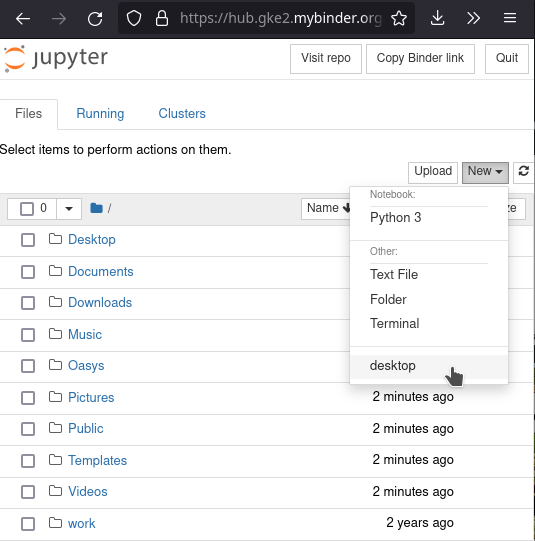
\includegraphics{figures/jupyter_select_desktop.png}
        \caption{}
        \label{fig:jupyter_select}
    \end{subfigure}
    \hfil
    \begin{subfigure}{0.5\textwidth}
        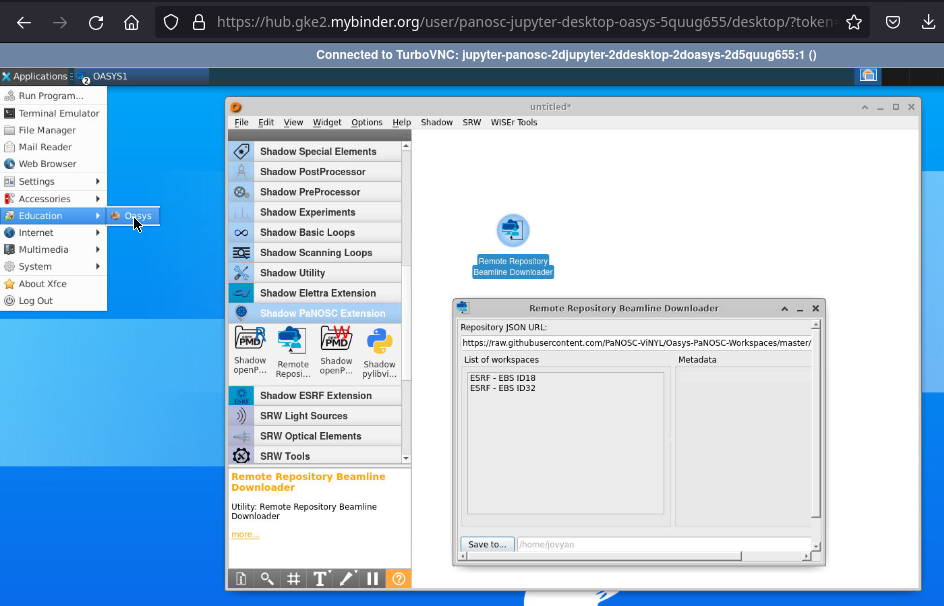
\includegraphics{figures/jupyter_oasys_run.png}
        \caption{}
        \label{fig:oasys_run}
    \end{subfigure}% trailing space between `subfigure` environments  had to be removed
    \caption{(a) Running the XFCE desktop environment from within Jupyter hub. (b) A new browser tab opens with XFCE desktop, providing a way to run OASYS inside the web browser while sharing the computing resources with the Jupyter hub instance.}
    \label{fig:oasysJupyter}
\end{figure}
The database itself consists of the actual OWS files and an index file and is hosted on Github. Since OWS files contain binary parts it is desirable not to change their content. Therefore an index file in JSON format is provided, serving two purposes:
\begin{itemize}
    \item user needs no Github account for read access,
    \item additional metadata can be provided.
\end{itemize}

\begin{table}[ht]
  \centering
  \caption{Oasys workspaces}
  \label{tab:oasys_workspaces}
  \begin{center}
    \begin{tabular}{ll}
      \hline
      OASYS workspaces database & \url{https://github.com/PaNOSC-ViNYL/Oasys-PaNOSC-Workspaces} \\
      OASYS Panosc toolbox code & \url{https://github.com/PaNOSC-ViNYL/OASYS1-PaNOSC} \\
      \hline
    \end{tabular}
  \end{center}
\end{table}


The index
file\footnote{\url{https://github.com/PaNOSC-ViNYL/Oasys-PaNOSC-Workspaces/blob/master/mainList.json}}
needs to be curated by the database admin and its changes can be easily tracked
through the git commits. Furthermore, this way the widget offers the possibility
of interacting with a database of arbitrary file formats and arbitrary
locations, while still retaining the metadata. Figure \ref{fig:oasys_database}
shows a screenshot of the widget. The links to the respective repositories are
listed in Table~\ref{tab:oasys_workspaces}.

Currently, two ESRF beamlines are ingested into the database and serve as the template for growing the repository.

\begin{figure}[ht]
    \centering
    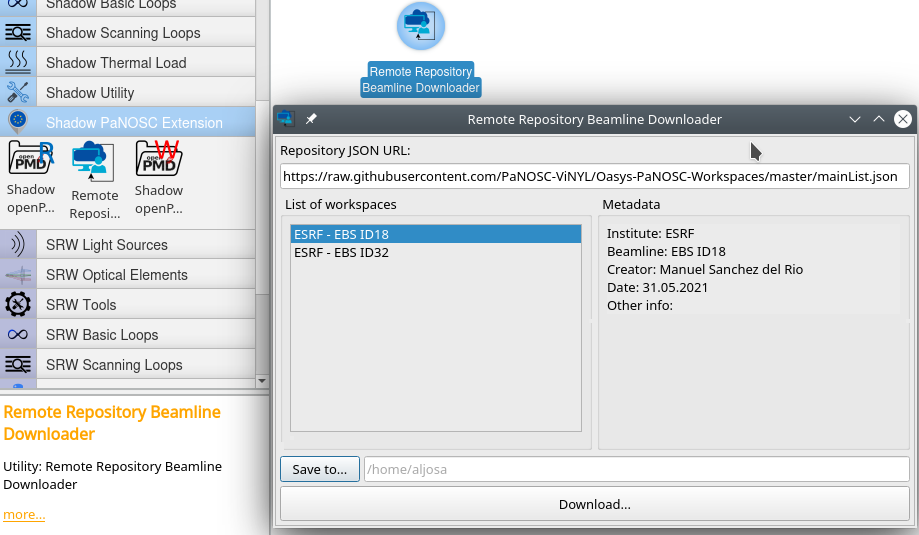
\includegraphics[width=0.52\textwidth]{figures/oasys_database_widget.png}
    \caption{OASYS widget for interaction with the online instrument database.}
    \label{fig:oasys_database}
\end{figure}

\section{McStasScript notebooks}
\label{sec:mcstas}
The McStasScript notebook repository and the code repository are listed
in Table~\ref{tab:mcstasscript_resources}.
\begin{table}[ht]
  \centering
  \caption{McStasScript resources}
  \begin{center}
    \begin{tabular}{ll}
      \hline
      McStasScript code repo  & \url{https://github.com/PaNOSC-ViNYL/McStasScript} \\ 
      McStasScript notebooks & \url{https://github.com/PaNOSC-ViNYL/McStasScript-notebooks} \\  
      McStasScript documentation & \url{https://mads-bertelsen.github.io}\\
      \hline
    \end{tabular}
  \end{center}
  \label{tab:mcstasscript_resources}
\end{table}
The McStasScript notebook repository currently contains a full 11 notebook
tutorial on McStas using the McStasScript Python interface developed under WP5.
This tutorial is also available through the online McStasScript documentation.
The repository also contains an example on using the widget interface for
McStasScript, and an example on using a cryostat construction tool included in
McStasScript.

\section{SimEx notebooks}
\label{sec:simex}
Numerous notebooks have been developed that showcase the use of the SIMEX
library for simulation of photon experiments at x--ray laser facilities. The
following table gives an overview and links directly to a static version of the
notebooks on github. 
To run these notebooks, a working SIMEX installation is needed.

% \begin{sidewaystable}[ht]
\begin{table}[ht]
  \caption{SIMEX notebooks}
  \begin{tabular}{l|p{9.8cm}}
    \hline
    \textbf{Notebook title} (link) & \textbf{Description} \\
    \hline
    \href{https://github.com/PaNOSC-ViNYL/SimEx-notebooks/blob/main/ESRF-SerialCrystallography/Jungfrau-ESRF.ipynb}{Jungfrau-ESRF.ipynb} & Crystallograhy at ESRF with 4M Jungfrau detector\\
    \href{https://github.com/PaNOSC-ViNYL/SimEx-notebooks/blob/main/SFX/crystFEL.ipynb}{crystFEL.ipynb} &  Nanocrystal diffraction at Eu.XFEL SFX instrument \\
    \href{https://github.com/PaNOSC-ViNYL/SimEx-notebooks/blob/main/SPB/diffrChaperonins.ipynb}{diffrChaperonins.ipynby} & Singe particle imaging at Eu.XFEL SPB instrument\\
    \href{https://github.com/PaNOSC-ViNYL/SimEx-notebooks/blob/main/s2e/start_to_end_demo.ipynb}{start\_to\_end\_demo.ipynb} & Start--to--end simulation for single particle imaging at Eu.XFEL SPB instrument. \\
    \href{https://github.com/PaNOSC-ViNYL/wavefrontDB/blob/main/examples/EuXFEL_SASE1_SPB_KBfocus.ipynb}{EuXFEL\_SASE1\_SPB\_KBfocus.ipynb} & KB mirror focusing of SASE1 beam at Eu.XFEL \\
    \href{https://github.com/PaNOSC-ViNYL/wavefrontDB/blob/main/examples/crl_focus.ipynb}{crl\_focus.ipynb} & CRL focusing of SASE1 beam at Eu.XFEL \\
    \href{https://github.com/PaNOSC-ViNYL/wavefrontDB/blob/main/examples/edge.ipynb}{edge.ipynb} & Coherent x--ray diffraction from a solid edge \\
    \href{https://github.com/PaNOSC-ViNYL/wavefrontDB/blob/main/examples/spheres.ipynb}{spheres.ipynb} & Coherent x--ray diffraction from solid spheres \\
    \href{https://github.com/PaNOSC-ViNYL/wavefrontDB/blob/main/examples/wire.ipynb}{wire.ipynb} & Coherent x--ray diffraction from a thin wire \\
    \hline
  \end{tabular}
  \label{tab:simex-notebooks}
\end{table}
% \end{sidewaystable}

% \printbibliography

% \fancypagestyle{plain}{}

\end{document}
